%% For double-blind review submission, w/o CCS and ACM Reference (max submission space)
\documentclass[sigplan,10pt,review,anonymous]{acmart}\settopmatter{printfolios=true,printccs=false,printacmref=false}
%% For double-blind review submission, w/ CCS and ACM Reference
%\documentclass[sigplan,10pt,review,anonymous]{acmart}\settopmatter{printfolios=true}
%% For single-blind review submission, w/o CCS and ACM Reference (max submission space)
%\documentclass[sigplan,10pt,review]{acmart}\settopmatter{printfolios=true,printccs=false,printacmref=false}
%% For single-blind review submission, w/ CCS and ACM Reference
%\documentclass[sigplan,10pt,review]{acmart}\settopmatter{printfolios=true}
%% For final camera-ready submission, w/ required CCS and ACM Reference
%\documentclass[sigplan,10pt]{acmart}\settopmatter{}


%% Conference information
%% Supplied to authors by publisher for camera-ready submission;
%% use defaults for review submission.
\acmConference[REBLS'18]{ACM SIGPLAN Workshop on Reactive and Event-Based Languages and Systems}{November 04, 2018}{Boston, MA, USA}
\acmYear{2018}
\acmISBN{} % \acmISBN{978-x-xxxx-xxxx-x/YY/MM}
\acmDOI{} % \acmDOI{10.1145/nnnnnnn.nnnnnnn}
\startPage{1}

%% Copyright information
%% Supplied to authors (based on authors' rights management selection;
%% see authors.acm.org) by publisher for camera-ready submission;
%% use 'none' for review submission.
\setcopyright{none}
%\setcopyright{acmcopyright}
%\setcopyright{acmlicensed}
%\setcopyright{rightsretained}
%\copyrightyear{2017}           %% If different from \acmYear

%% Bibliography style
\bibliographystyle{ACM-Reference-Format}
%% Citation style
%\citestyle{acmauthoryear}  %% For author/year citations
%\citestyle{acmnumeric}     %% For numeric citations
%\setcitestyle{nosort}      %% With 'acmnumeric', to disable automatic
                            %% sorting of references within a single citation;
                            %% e.g., \cite{Smith99,Carpenter05,Baker12}
                            %% rendered as [14,5,2] rather than [2,5,14].
%\setcitesyle{nocompress}   %% With 'acmnumeric', to disable automatic
                            %% compression of sequential references within a
                            %% single citation;
                            %% e.g., \cite{Baker12,Baker14,Baker16}
                            %% rendered as [2,3,4] rather than [2-4].


%%%%%%%%%%%%%%%%%%%%%%%%%%%%%%%%%%%%%%%%%%%%%%%%%%%%%%%%%%%%%%%%%%%%%%
%% Note: Authors migrating a paper from traditional SIGPLAN
%% proceedings format to PACMPL format must update the
%% '\documentclass' and topmatter commands above; see
%% 'acmart-pacmpl-template.tex'.
%%%%%%%%%%%%%%%%%%%%%%%%%%%%%%%%%%%%%%%%%%%%%%%%%%%%%%%%%%%%%%%%%%%%%%


%% Some recommended packages.
\usepackage{booktabs}   %% For formal tables:
                        %% http://ctan.org/pkg/booktabs
\usepackage{subcaption} %% For complex figures with subfigures/subcaptions
                        %% http://ctan.org/pkg/subcaption

\usepackage{xspace}
\newcommand{\CEU}{\textsc{C\'{e}u}\xspace}

\newcommand{\code}[1] {{\small{\texttt{#1}}}}

\usepackage{listings}
\lstdefinelanguage{ceu}{%
  language=C,
  morekeywords={%
    @const, @pure, @safe, NEVER, FOREVER, PAR, PROC, SIGNAL, abort, and,
    await, bool, call, class, data, define, deterministic, do, each, else,
    emit, end, escape, event, every, finalize, hor, implementation, in,
    input, interface, loop, min, native, new, nohold, not, or, output, par,
    pool, pure, return, s, h, ms, signal, spawn, tag, then, this, traverse, until,
    code, public, private,
    var, watching, when, with},
}
\lstset{
  literate={~} {$\sim$}{1},
  basicstyle=\footnotesize\ttfamily,
  captionpos=b,
  columns=flexible,
  commentstyle=\footnotesize\itshape,
  escapeinside={||},
  frame=tb,
  keepspaces=true,
  keywordstyle=\bfseries,
  language=ceu,
  mathescape=true,
  numbersep=4pt,
  numberstyle=\tiny,
  %xleftmargin=0.5cm,
  %xrightmargin=0.5cm,
  %upquote=true,
}

\usepackage{tikz}
\usetikzlibrary{
  arrows,
  arrows.meta,
  calc,
  decorations.pathreplacing,
  decorations.text,
  math,
  positioning,
  shapes,
}

\begin{document}

%% Title information
\title{Where Do Events Come From?}
\subtitle{Reactive Programming From The Ground Up}

%% Author information
%% Contents and number of authors suppressed with 'anonymous'.
%% Each author should be introduced by \author, followed by
%% \authornote (optional), \orcid (optional), \affiliation, and
%% \email.
%% An author may have multiple affiliations and/or emails; repeat the
%% appropriate command.
%% Many elements are not rendered, but should be provided for metadata
%% extraction tools.

%% Author with single affiliation.
\author{First1 Last1}
\authornote{with author1 note}          %% \authornote is optional;
                                        %% can be repeated if necessary
\orcid{nnnn-nnnn-nnnn-nnnn}             %% \orcid is optional
\affiliation{
  \position{Position1}
  \department{Department1}              %% \department is recommended
  \institution{Institution1}            %% \institution is required
  \streetaddress{Street1 Address1}
  \city{City1}
  \state{State1}
  \postcode{Post-Code1}
  \country{Country1}                    %% \country is recommended
}
\email{first1.last1@inst1.edu}          %% \email is recommended

%% Author with two affiliations and emails.
\author{First2 Last2}
\authornote{with author2 note}          %% \authornote is optional;
                                        %% can be repeated if necessary
\orcid{nnnn-nnnn-nnnn-nnnn}             %% \orcid is optional
\affiliation{
  \position{Position2a}
  \department{Department2a}             %% \department is recommended
  \institution{Institution2a}           %% \institution is required
  \streetaddress{Street2a Address2a}
  \city{City2a}
  \state{State2a}
  \postcode{Post-Code2a}
  \country{Country2a}                   %% \country is recommended
}
\email{first2.last2@inst2a.com}         %% \email is recommended
\affiliation{
  \position{Position2b}
  \department{Department2b}             %% \department is recommended
  \institution{Institution2b}           %% \institution is required
  \streetaddress{Street3b Address2b}
  \city{City2b}
  \state{State2b}
  \postcode{Post-Code2b}
  \country{Country2b}                   %% \country is recommended
}
\email{first2.last2@inst2b.org}         %% \email is recommended


%% Abstract
%% Note: \begin{abstract}...\end{abstract} environment must come
%% before \maketitle command

\begin{abstract}
In reactive and event-based systems, execution is guided by an external
environment which generates inputs to the application and consumes outputs from
it.
Reactive languages provide dedicated syntax and semantics to deal with events
and greatly simplify the programming experience in this domain.
%
Nevertheless, the environment is typically prefabricated in a host language and
the very central concept of events is implemented externally to the reactive
language.
%
In this work, we propose an interrupt handler primitive for a reactive language
targeting embedded systems in order to take control of the whole event loop,
from a sensor input source and back to an actuator output.
%
We propose the new asynchronous primitive in the context of the synchronous
language \CEU and discuss how they synergize to avoid race conditions at
compile time, support lexically-scoped drivers, and provide automatic standby
for applications.
%and hot swapping of device drivers
\end{abstract}

%% 2012 ACM Computing Classification System (CSS) concepts
%% Generate at 'http://dl.acm.org/ccs/ccs.cfm'.
\begin{CCSXML}
<ccs2012>
<concept>
<concept_id>10011007.10011006.10011008</concept_id>
<concept_desc>Software and its engineering~General programming languages</concept_desc>
<concept_significance>500</concept_significance>
</concept>
<concept>
<concept_id>10003456.10003457.10003521.10003525</concept_id>
<concept_desc>Social and professional topics~History of programming languages</concept_desc>
<concept_significance>300</concept_significance>
</concept>
</ccs2012>
\end{CCSXML}

\ccsdesc[500]{Software and its engineering~General programming languages}
\ccsdesc[300]{Social and professional topics~History of programming languages}
%% End of generated code


%% Keywords
%% comma separated list
\keywords{interrupt service routine,
          sleep mode,
          synchronous reactive programming}

\maketitle

\section{Introduction}

Reactive applications interact continuously and in real time with the external
world through sensors and actuators (e.g., buttons, displays, timers, etc.).
%
These interactions are typically represented as input events flowing from the
devices to the application and as output events flowing from the application to
the devices.
%
As illustrated in Figure~\ref{fig.env}, devices can be encapsulated as a
single component, \emph{the environment}, which controls the system execution
in an event loop:
the application sits idle waiting for an input;
the environment awakes the application on the occurrence of an input;
the application reacts to the input and generates back one or more outputs;
the application becomes idle and the loop restarts.

\begin{figure}
\centering
\includegraphics[width=\linewidth]{loop}
\caption{ Event loop in reactive systems.
          The environment controls the application through input \& output
          events.
\label{fig.env}
}
\end{figure}

The environment is typically implemented in a host language (e.g., C) and
controls the main event loop, invoking entry points in the reactive language
runtime on the occurrence of inputs and also receiving output calls, both
through a documented API.
%
As examples, Esterel~\cite{esterel.ieee91} relies on C for passing events
between the environment and the running program~\cite{esterel.book.compiling},
while Elm~\cite{frp.elm} uses the concept of \emph{ports}, which allows sending
out values to JavaScript in commands and listening for values in
subscriptions~\cite{frp.elm.ports}.

The event-based interface between the application and the environment is
arguably inevitable and also happens at the right level of abstraction, since
it connects the application with the operating system resources through a
non-invasive API.
%
However, this separation exposes the environment as a rigid system component
that evolves in separate from the application.
%
It also requires two languages and the programmer has to deal with multiple
syntaxes, incompatible type systems, and different address spaces.
%
Furthermore, in the context of embedded systems, a proper host OS may even be
absent or lacking enough device drivers, which requires more low-level
intervention from the application.

In this work, we propose interrupt service routines (ISRs) as an asynchronous
primitive for the synchronous language \CEU~\cite{ceu.sensys13}.
ISRs empower applications to also implement their own device drivers and
self-generate inputs, bypassing the need for a host environment.
%
\CEU targets resource-constrained architectures, such as Arduino-compatible
microcontrollers, in which applications run in the bare metal, without
operating system support.
In this context, device drivers are typically libraries compiled together with
the main program.

The lack of an OS opens an opportunity to explore a tighter integration between
the application and its device drivers at the language level, resulting in an
overall simplicity and tractability of the system.
%
In particular, \CEU is amenable to a simple static analysis to detect race
conditions that we extended to encompass ISRs.
%
\CEU also provides a lexical finalization mechanism that we adopt in drivers to
properly disable interrupts.
%
Finally, the synchronous semantics of \CEU enforces that applications react
to inputs in bounded time and remain in an idle states susceptible to standby.
With the help of drivers and a power management runtime, \CEU can put the
microcontroller to sleep automatically at optimal sleeping modes after each
input reaction.

We implemented an extensible runtime that exposes hooks for the interrupts and
the power manager, which we validated in two microcontrollers: an
\emph{8-bit AVR/ATmega} and a \emph{32-bit ARM/Cortex-M0}.
%
We also implemented drivers for a variety of peripherals, such as GPIO, A/D
converter, USART, SPI, and nRF24L01 transceiver.
%
Applications can share data buffers with drivers to avoid unnecessary copying,
with the static guarantee that no data races will occur.
%
We demonstrate that applications built on top of these drivers show significant
energy savings due to automatic standby.

TODO: weakness

what would be

output (int,int) O;

becomes

output (int x, int y) O do
end

\begin{comment}
% Esterel
https://books.google.com.br/books?id=O5zi14i0KP4C&pg=PA31&lpg=PA31&dq=esterel+external+signal+api&source=bl&ots=43EBAqIkSJ&sig=npYylZteOmZAqv4f7SXAtJO9xr8&hl=en&sa=X&ved=0ahUKEwjFlf7-3p_cAhWPrVkKHXsFDWgQ6AEIUjAG#v=onepage&q=esterel%20external%20signal%20api&f=false
Esterel relies on general-purpose languages such as C or C++ in two ways.       
First, for portability, most Esterel compilers generate C instead of            
assembly or some other executable representation.                               
Such generated code provides an interface for passing events between the        
environment and the running program.                                            
Second, Esterel allows the use of data types and functions defined externally   
(e.g., in C) to be used within an Esterel program.                              

% Elm
https://guide.elm-lang.org/interop/javascript.html
Okay, in Elm, any communication with JavaScript goes through a port. Think of
it like a hole in the side of your Elm program where you can send values in and
out. These work exactly like the commands and subscriptions from the
Architecture section. Sending values out to JS is a command. Listening for
values coming in from JS is a subscription. Pretty neat!
\end{comment}

- excel define formulas for input but not the input itself

output -> input

the environment sits
    inverse
    reacts to output and generates inputs

remain idle and react to the occurrence of events 


\section{\CEU: Structured Synchronous Reactive Programming}
\label{sec.ceu}

\CEU is a Esterel-based~\cite{ceu.tecs17} reactive programming language
targeting resource-constrained embedded systems~\cite{ceu.sensys13}, with the
characteristics that follow:
%
\begin{description}
\item [Reactive:] code only executes in reactions to events and is idle most of
    the time.
\item [Structured:] programs use lexically-scoped structured control
    mechanisms, such as \code{await} (to suspend a line of execution), and
    \code{par} (to combine multiple lines of execution).
\item [Synchronous:] reactions run atomically and to completion on each line of
    execution, i.e., there's no implicit preemption or real parallelism.
\end{description}

Structured reactive programming lets developers write code in direct style,
recovering from the inversion of control imposed by event-driven
execution~\cite{rp.deprecating,rp.rescala,sync_async.cooperative}.

\begin{lstlisting}[
  xleftmargin=1em,
  numbers=left,
  basicstyle=\ttfamily\small,
  float=h,
  caption={A \CEU program that toggles the state of the LED whenever a radio
           packet is received, terminating on a button press, always with the
           LED off.},
  label={lst.ceu},
]
output high/low LED;
input  high/low BUTTON;
input  Packet   RADIO_RECV;
par/or do
    var high/low v = await BUTTON (until v==low);
with
    finalize with
        emit LED(low);
    end
    loop do
        emit LED(high);
        await RADIO_RECV;
        emit LED(low);
        await RADIO_RECV;
    end
end
\end{lstlisting}

The example in Listing~\ref{lst.ceu} illustrates the main characteristics of
\CEU, namely event-driven I/O, lexically-scoped compositions and synchronous
execution.
%
The program toggles the state of the LED whenever a radio packet is received,
terminating on a button press, always with the LED off.
%
The program first declares the \code{LED} output, and the \code{BUTTON} and
\code{RADIO\_RECV} input events (ln~1--3).
The declarations include a payload type, i.e., each event occurrence carries
a value of that type (\code{high/low} is a boolean type).
%
Then, the program uses a \code{par/or} composition to run two lines of
execution, aka \emph{trails}, in parallel:
a single-statement trail that waits for a button press before terminating
(ln~5), and an endless loop that toggles the LED on and off whenever a radio
packet is received (ln~10--15).
Since we care about any reception occurrence, the example ignores the actual
packet payload (ln~12,14).
The \code{finalize} clause (ln~7--9) ensures that, no matter how its enclosing
trail terminates, the LED will be unconditionally turned off~(ln~8).

All communication between the application and the environment is done through
the \code{await} and \code{emit} primitives, which awaits an input event and
generates an output event, respectively.

The \code{par/or}, which stands for \emph{parallel-or}, is a lexical
composition that terminates as soon as one of the trails terminates, but which
also automatically finalizes the other trail(s).
%
In the example, when the button is pressed, not only the toggling loop will be
aborted, but the \code{finalize} clause will turn the LED off unconditionally,
since its enclosing block went out of scope.

The synchronous execution model of \CEU dictates that reactions to input events
are atomic and that incoming events are never lost.
%
The event loop in Figure~\ref{fig.env} indicates this behavior since the
environment can only generate a new input after the application yields control
and closes the loop.
%
In the example, even if two packets arrive simultaneously in the environment,
the synchronous model provides the atomicity and responsiveness guarantees:
    the first \code{await} will awake and turn the LED off atomically
    (ln 12--13);
    and the second \code{await} will awake in sequence (ln 14).
%
%Note that if multiple trails in parallel await the same input, they will all
%awake from it during the same reaction.
%In this case, \CEU dictates that each trail executes atomically, one after the
%other, in lexical order.
%This rule prevents race conditions for trails in parallel.

Figure~\ref{fig.ticks} illustrates the synchronous execution model of \CEU.
%
The continuous timeline in the environment shows an absolute reference clock
with ``physical timestamps'' for the event occurrences (e.g., event~\code{C}
occurs at 17ms521us).
%
The discrete timeline in the application shows how the same occurring events
fit in the logical notion of time of \CEU.
%
The boot reaction \code{boot-0} happens before any input, at program startup.
%
Event~\code{A} ``physically'' occurs during \code{boot-0} but, because time
is discrete, its corresponding reaction only executes afterwards, at logical
instant~\code{A-1}.
%
Similarly, event~\code{B} occurs during~\code{A-1} and its reaction is
postponed to execute at~\code{B-2}.
%
Event~\code{C} also occurs during~\code{A-1} but its reaction must also wait
for~\code{B-2} to execute and so it is postponed to execute at~\code{C-3}.
%
Finally, event~\code{D} occurs during an idle period and can start immediately
at \code{D-4}.
%
%Finally, two instances of event~\code{E} occur during~\code{D-4}; they are
%handled in the subsequent reactions~\code{E-5} and~\code{E-6}.

\begingroup
\begin{figure}[t]
\centering
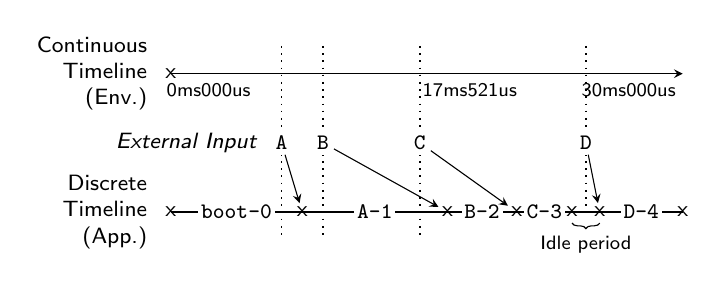
\begin{tikzpicture}[x=1em,y=1em,
  font=\footnotesize\sffamily,>=stealth,
  time/.style={font=\scriptsize\sffamily},
  cross/.style={inner sep=0pt,outer sep=0pt},
  evt/.style={fill=white,inner sep=1.85pt,outer sep=0pt},
  rng/.style={fill=white,inner sep=1pt,outer sep=0pt,
    font=\ttfamily\footnotesize}]
  \draw[->]
  (0,0)
    node[align=right,anchor=east,xshift=-.5em]
        {Continuous\\Timeline\\(Env.)}
    node[anchor=north west,xshift=-.5em,time]
        {0ms000us}
    node[anchor=north west,xshift=8.75em,time]
        {17ms521us}
  -- (18.5,0)
    node[anchor=north east,xshift=.1em,time]
        {30ms000us};
  \node[cross] at (0,0){x};
  %%
  \coordinate(Ext) at ($(0,0)!.5!(0,-5)$);
  \coordinate(A) at (Ext-|4,0);
  \coordinate(B) at (Ext-|5.5,0);
  \coordinate(C) at (Ext-|9,0);
  \coordinate(D) at (Ext-|15,0);
  %%
  \draw[semithick,dotted] (0,1-|A) -- (0,-6-|A);
  \draw[semithick,dotted] (0,1-|B) -- (0,-6-|B);
  \draw[semithick,dotted] (0,1-|C) -- (0,-6-|C);
  \draw[semithick,dotted] (0,1-|D) -- (0,-5-|D);
  \node[evt](Aevt) at (A) {\texttt{\textbf{A}}};
  \node[evt](Bevt) at (B) {\texttt{\textbf{B}}};
  \node[evt](Cevt) at (C) {\texttt{\textbf{C}}};
  \node[evt](Devt) at (D) {\texttt{\textbf{D}}};
  \node[anchor=east,xshift=-.5em] at (A){\emph{External Input}};
  %%
  \draw[-]
  (0,-5)
    node[align=right,anchor=east,xshift=-.5em]
        {Discrete\\Timeline\\(App.)}
  -- (18.5,-5);
  \node[cross](P0) at (0,-5){x};
  \node[cross](P1) at (4.75,-5){x};
  \node[cross](P2) at (10,-5){x};
  \node[cross](P3) at (12.5,-5){x};
  \node[cross](P4) at (14.5,-5){x};
  \node[cross](P5) at (15.5,-5){x};
  \node[cross](P6) at (18.5,-5){x};
  \node[rng] at ($(P0)!.5!(P1)$){boot-0};
  \node[rng] at ($(P1)!.5!(P2)$){A-1};
  \node[rng] at ($(P2)!.5!(P3)$){B-2};
  \node[rng] at ($(P3)!.5!(P4)$){C-3};
  \node[rng] at ($(P5)!.5!(P6)$){D-4};
  \draw[decorate,decoration={brace,raise=-1pt,mirror,amplitude=2pt}]
  ($(P4)+(0,-.5)$) -- node[below,time] {Idle period} ($(P5)+(0,-.5)$);
  %%
  \begin{scope}[shorten >=1.5pt]
  \draw[->] (Aevt) -- (P1);
  \draw[->] (Bevt) -- (P2);
  \draw[->] (Cevt) -- (P3);
  \draw[->] (Devt) -- (P5);
  \end{scope}
\end{tikzpicture}
\vskip-.6em
%\includegraphics[width=\columnwidth]{tick_min}
\caption{The discrete notion of time in \CEU.}
\label{fig.ticks}
\end{figure}
\endgroup


In order to guarantee responsiveness, the synchronous model relies on the
\emph{synchronous hypothesis}, which states that reactions must be
significantly faster than the rate of inputs.
%
For this reason, \CEU (like most synchronous languages) restricts itself and
refuses unbounded loops at compile time.
This guarantees that all reactions to the environment are computed in bounded
time~\cite{ceu.lctes18}, ensuring that applications are always responsive to
incoming events.

\section{Interrupt Service Routines in \CEU}
\label{sec.isrs}

Interrupts service routines (ISRs) are software entry points that execute in
response to hardware interrupts from peripherals such as timers and GPIOs.
ISRs are at the lowest level interface between hardware and software and are
the absolute source of inputs to programs.
%
Typically, an ISR starts to execute as soon as the hardware interrupt occurs
and suspends the normal program flow abruptly.
Such asynchronous behavior reflects the inherent concurrent nature of
peripherals interacting with the external world.

\begin{figure}
\centering
\includegraphics[width=\linewidth]{sync-async}
\caption{ An application in \CEU has a concurrent asynchronous side and a
          predictable synchronous side that receives and reacts to inputs
          atomically.
\label{fig.async}
}
\end{figure}

Asynchronous execution confronts the synchronous mindset of \CEU since the
assumption that reactions are atomic no longer holds.
Not only this may lead to race conditions at a fine grain, but may also affect
the ordering of events at a coarse grain: the effect of an earlier event may be
perceived after the effect of a later event.
%
Nevertheless, our goal is to preserve the well-behaved interaction between the
\CEU application and the environment as of Figure~\ref{fig.env}, even in the
presence of asynchronous ISRs as illustrated in Figure~\ref{fig.async}:
%
the original application is now represented by the synchronous \CEU and the
environment by the asynchronous \CEU, all inside the same application.
%
This way, we want to push all subtleties of asynchronous execution into device
drivers which emit input events to regular synchronous code in \CEU exactly
as before.

\begin{lstlisting}[
  xleftmargin=1em,
  numbers=left,
  basicstyle=\ttfamily\small,
  float=t,
  caption={XXX.},
  label={lst.gpio.sync},
  escapechar=\%,
]
output high/low PIN_13;
input  high/low PIN_02;
#include "gpio.ceu"

emit PIN_13(low);
loop do
    var high/low v = await PIN_02;
    emit PIN_13(v);
end
\end{lstlisting}

\begin{lstlisting}[
  xleftmargin=1em,
  numbers=left,
  basicstyle=\ttfamily\small,
  float=t,
  caption={XXX.},
  label={lst.gpio.async},
  escapechar=\%,
]
// OUTPUT DRIVER

{ pinMode(13, OUTPUT); }
output (high/low v) PIN_13 do
    { digitalWrite(13, @v); }
end

// INPUT DRIVER

input high/low PIN_02;
{
    pinMode(2, INPUT_PULLUP);
    EICRA = (EICRA & ~((1<<ISC00) | (1<<ISC01)))
          | (CHANGE << ISC00);
    EIMSK |= (1<<INT0);
}
spawn async/isr [INT0_vect] do
    emit PIN_02({digitalRead(2)});
end
\end{lstlisting}

Listing~\ref{lst.gpio.sync}~and~\ref{lst.gpio.async} implements an application
that uses GPIO to link a button (pin 02) to an LED (pin 13) such that the LED
is on whenever the button is pressed.
%
The synchronous side (Listing~\ref{lst.gpio.sync}) declares its interface with
the external world and includes the asynchronous side as a driver (ln 1--3).
%
The asynchronous side (Listing~\ref{lst.gpio.async}) implements the output and
input events.

An \code{output} implementation (ln 4--6) is similar to a parameterized
subroutine: whenever the application invokes \code{emit}, the output body
executes atomically.
\CEU supports inline C between curly braces (ln 3,5) with interpolation to
evaluates \CEU expressions (e.g., \code{@v}).
This allows drivers to take advantage of existing libraries in embedded
toolchains, such as Arduino.
%
In the example, the driver sets pin 13 as output (ln 3) when it is included,
and sets its state whenever it is emitted (ln 5).

An \code{input} event implementation requires an ISR registered with the
\code{spawn async/isr} primitive (ln 17--19), which is automatically invoked
whenever the associated interrupt occurs (e.g., \code{INT0\_vect}).
%
An ISR in \CEU will always have an \code{emit} to an input event inside its
body to awake the synchronous side.
However, although the ISR executes asynchronously as soon as the interrupt
occurs, the \code{emit} respects the semantics of \CEU and does not interrupt
an ongoing reaction on the synchronous side.
%
In the example, the input driver first configures pin 2 to behave as input and
to generate an external interrupt on level transitions (ln 11--16).

synchronous remains simple and well behaved
with no low-level calls





The application only communicates


- finite is can be still much greater than 0 (order of milliseconds)
    - which is a lot of time

%% Acknowledgments
\begin{acks}                            %% acks environment is optional
                                        %% contents suppressed with 'anonymous'
  %% Commands \grantsponsor{<sponsorID>}{<name>}{<url>} and
  %% \grantnum[<url>]{<sponsorID>}{<number>} should be used to
  %% acknowledge financial support and will be used by metadata
  %% extraction tools.
  This material is based upon work supported by the
  \grantsponsor{GS100000001}{National Science
    Foundation}{http://dx.doi.org/10.13039/100000001} under Grant
  No.~\grantnum{GS100000001}{nnnnnnn} and Grant
  No.~\grantnum{GS100000001}{mmmmmmm}.  Any opinions, findings, and
  conclusions or recommendations expressed in this material are those
  of the author and do not necessarily reflect the views of the
  National Science Foundation.
\end{acks}


%% Bibliography
\bibliography{my,other}


%% Appendix
\appendix
\section{Appendix}

Text of appendix \ldots

\end{document}
